\documentclass{beamer}

\usepackage{epsfig}
\usepackage{multicol}
\usepackage{geometry}
%\usepackage[dvipsnames]{xcolor}
\usepackage{textcomp}
\usepackage{graphicx}
\usepackage{caption}
\usepackage{subcaption}
\usepackage{amsmath}
\usepackage{tcolorbox}
\usetheme{Boadilla}
\usepackage{pict2e}
\usepackage{tikz}
\usepackage{xcolor}


\title[Traitement du signal numérique]{Traitement du signal numérique - HEI4 IMS}
\author[Antony Bazir]{}

\setlength{\unitlength}{1cm}

\begin{document}
\section{Rappel}
\begin{frame}
\frametitle{Rappels : Signaux }
\textbf{Signal numérique =  codage + échantillonnage}
\begin{center}
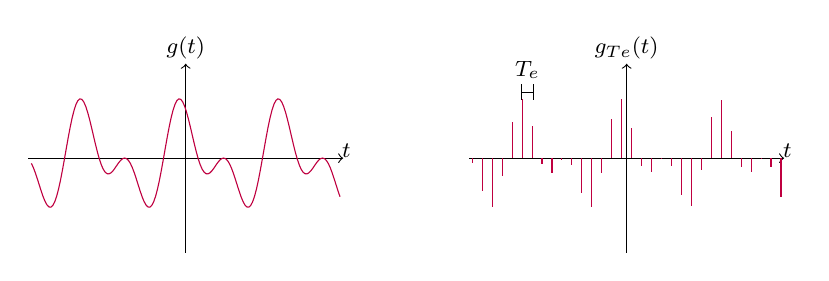
\begin{tikzpicture}
\begin{scope}[scale=0.4]
	\draw[->] (-5,0)-- (5,0);
%\draw (-0.3,-0.3) node {0};
\draw[->] (0,-3)-- (0,3);
\draw (5.1,0.25) node {\footnotesize{$t$}};
\draw (0,3.5) node {\footnotesize{$g(t)$}};
%\draw (4.5,-0.3) node {1};

\draw[domain=-4.9:4.9,color=purple,samples=160] plot (\x,{2*(0.55*cos(2*\x r)+ 0.45*cos(2*2*(\x+3.14/12) r))});
\end{scope}

\begin{scope}[scale=0.4,xshift=14cm]
	\draw[->] (-5,0)-- (5,0);
%\draw (-0.3,-0.3) node {0};
\draw[->] (0,-3)-- (0,3);
\draw (5.1,0.25) node {\footnotesize{$t$}};
\draw (0,3.5) node {\footnotesize{$g_{Te}(t)$}};
%\draw (4.5,-0.3) node {1};
\draw[|-|] (-2.95,2.1)--(-3.35,2.1);
\draw (-3.15,2.8) node {\footnotesize{$T_e$}};

\draw[domain=-4.9:4.9,color=purple,samples=32] plot[ycomb] (\x,{2*(0.55*cos(2*\x r)+ 0.45*cos(2*2*(\x+3.14/12) r))});
%\draw[domain=-4.9:4.9,dotted,color=purple,samples=32] plot[xcomb] (\x,{2*(0.55*cos(2*\x r)+ 0.45*cos(2*2*(\x+3.14/12) r))});
\end{scope}
	\end{tikzpicture}
\end{center}
\vspace{0.5cm}
\begin{itemize}
\item \'Echantillonage : discrétisation en temps
\vspace{0.3cm}
\item Codage : discrétisation en amplitude
\end{itemize}
\end{frame}

\begin{frame}
\frametitle{Rappel : Analyse de signaux}
Pour les signaux discrets on utilise TOUJOURS la transformée en Z
\[\boxed{TZ\{ f \}(z) = \sum_{n = -\infty}^{\infty} f[n] z^{-n}} \]
On en dérive la transformée de Fourier 
\[\boxed{TF\{ f \}(\nu) = \sum_{n = -\infty}^{\infty} f[n] e^{-j 2 \pi n \nu T_e}} \]
\vspace{0.2cm}
La transformée de Fourier donne ce qu'on appelle le \textbf{spectre fréquentiel/réponse en fréquence} d'un signal/système
\end{frame}

\begin{frame}
\frametitle{Rappel : Analyse de signaux}
Les spectres fréquentiels/réponses en fréquences sont \textbf{généralement complexes}
\begin{center}
\begin{tikzpicture}
\begin{scope}[scale=0.4]
	\draw[->] (-5,0)-- (5,0);
%\draw (-0.3,-0.3) node {0};
\draw[->] (0,-3)-- (0,3);
\draw (5.1,0.25) node {\footnotesize{$t$}};
\draw (0,3.5) node {\footnotesize{$g_{Te}(t)$}};
%\draw (4.5,-0.3) node {1};
\draw[|-|] (-2.95,2.1)--(-3.35,2.1);
\draw (-3.15,2.8) node {\footnotesize{$T_e$}};

\draw[domain=-4.9:4.9,color=purple,samples=32] plot[ycomb] (\x,{2*(0.55*cos(2*\x r)+ 0.45*cos(2*2*(\x+3.14/12) r))});
%\draw[domain=-4.9:4.9,dotted,color=purple,samples=32] plot[xcomb] (\x,{2*(0.55*cos(2*\x r)+ 0.45*cos(2*2*(\x+3.14/12) r))});
\end{scope}
	\end{tikzpicture}
\end{center}

\begin{columns}
\column{60mm}
\underline{\small{Réponse en amplitude (Module  TF)}}:\\
\begin{center}
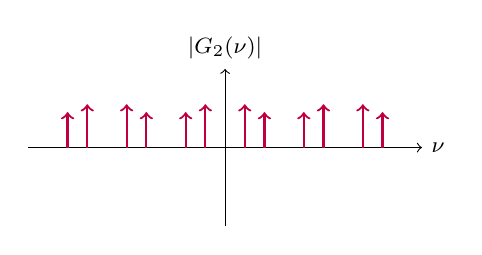
\begin{tikzpicture}
\begin{scope}
\draw[->] (-2.5,0)--(2.5,0) node[right]{\footnotesize{$\nu$}};
\draw[->] (0,-1)--(0,1) node[above]{\footnotesize{$|G_2(\nu)|$}};
\draw[->,purple,thick] (-1/4,0)--(-1/4,0.55) ;
\draw[->,purple,thick] (1/4,0)--(1/4,0.55) ;
\draw[->,purple,thick] (-2/4,0)--(-2/4,0.45) ;
\draw[->,purple,thick] (2/4,0)--(2/4,0.45) ;

\draw[->,purple,thick] (-1/4+1.5,0)--(-1/4+1.5,0.55) ;
\draw[->,purple,thick] (1/4+1.5,0)--(1/4+1.5,0.55) ;
\draw[->,purple,thick] (-2/4+1.5,0)--(-2/4+1.5,0.45) ;
\draw[->,purple,thick] (2/4+1.5,0)--(2/4+1.5,0.45) ;

\draw[->,purple,thick] (-1/4-1.5,0)--(-1/4-1.5,0.55) ;
\draw[->,purple,thick] (1/4-1.5,0)--(1/4-1.5,0.55) ;
\draw[->,purple,thick] (-2/4-1.5,0)--(-2/4-1.5,0.45) ;
\draw[->,purple,thick] (2/4-1.5,0)--(2/4-1.5,0.45) ;
\end{scope}
\end{tikzpicture}
\end{center}


\column{60mm}
\underline{\small{Réponse en phase (Argument TF)}}:\\
\begin{center}
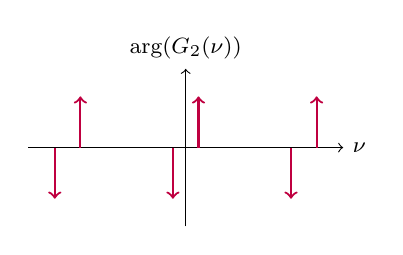
\begin{tikzpicture}
\begin{scope}
\draw[->] (-2,0)--(2,0) node[right]{\footnotesize{$\nu$}};
\draw[->] (0,-1)--(0,1) node[above]{\footnotesize{$\text{arg}(G_2(\nu))$}};
\draw[->,purple,thick] (-0.65/4,0)--(-0.65/4,-0.65) ;
\draw[->,purple,thick] (0.65/4,0)--(0.65/4,0.65) ;

\draw[->,purple,thick] (-0.65/4-1.5,0)--(-0.65/4-1.5,-0.65) ;
\draw[->,purple,thick] (0.65/4-1.5,0)--(0.65/4-1.5,0.65) ;

\draw[->,purple,thick] (-0.65/4+1.5,0)--(-0.65/4+1.5,-0.65) ;
\draw[->,purple,thick] (0.65/4+1.5,0)--(0.65/4+1.5,0.65) ;

\end{scope}
\end{tikzpicture}
\end{center}
\end{columns}

\end{frame}

\begin{frame}
\frametitle{}
\[TF\{ x \}(\nu) = \sum_{n = -\infty}^{\infty} x[n] e^{-j 2 \pi n \nu T_e} \]
La transformée de Fourier d'un signal discret n'est pas calculables par un ordinateur...\\
\vspace{0.6cm}
Transformée de Fourier \textbf{Discrète}
\[ TFD\{ x \}[m] = \frac{1}{N} \sum_{n = 0}^{N-1} x[n] \; e^{-j 2 \pi n \frac{m}{N}}  \] 
\vspace{0.3cm}
Approximation de la transformée de Fourier...
\end{frame}

\begin{frame}
\frametitle{}
\begin{center}
\begin{tikzpicture}
\begin{scope}[scale=0.4]
	\draw[->] (-5,0)-- (5,0);
%\draw (-0.3,-0.3) node {0};
\draw[->] (0,-3)-- (0,3);
\draw (5.1,0.25) node {\footnotesize{$t$}};
\draw (0,3.5) node {\footnotesize{$g_{Te}(t)$}};
%\draw (4.5,-0.3) node {1};
\draw[|-|] (-2.95,2.1)--(-3.35,2.1);
\draw (-3.15,2.8) node {\footnotesize{$T_e$}};

\draw[domain=-4.9:4.9,color=purple,samples=32] plot[ycomb] (\x,{2*(0.55*cos(2*\x r)+ 0.45*cos(2*2*(\x+3.14/12) r))});
%\draw[domain=-4.9:4.9,dotted,color=purple,samples=32] plot[xcomb] (\x,{2*(0.55*cos(2*\x r)+ 0.45*cos(2*2*(\x+3.14/12) r))});
\end{scope}
	\end{tikzpicture}
\end{center}
\end{frame}

\section{Application TFD}
\subsection{Introduction}
\begin{frame}
\frametitle{Introduction}
Rappel :  Définition transformée de Fourier discrète (TFD)\\
\vspace{0.3cm} 
\[ TFD\{ x \}[m] =  \sum_{k = 0}^{N-1} x[k] \; e^{-j 2 \pi k \frac{m}{N}}  \] \\
\vspace{0.3cm}
\only<2->{
\begin{itemize}
\item Somme finie sur les échantillons temporels
\vspace{0.1cm}
\item Nombre fini de valeurs de fréquence
\end{itemize}
}
 
\only<3->{
\vspace{0.5cm}
On va prendre des exemples de signaux simples pour illustrer clairement certains aspects techniques et le lien avec la transformée de Fourier
}
\end{frame}

\begin{frame}
\frametitle{Signal porte} 
On prend l'exemple du signal porte 
\begin{columns}
\column{60mm}
\begin{center}
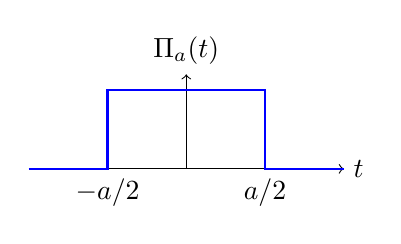
\begin{tikzpicture}
\draw[->] (0,0)--(0,1.2)node[above]{$\Pi_a (t)$}; 
\draw[->] (-2,0)--(2,0)node[right]{$t$};  

\draw[blue,thick] (-2,0)--(-1,0)node[black,below] {$-a/2$}--(-1,1)--(1,1)--(1,0)node[black,below] {$a/2$}--(2,0); 
\end{tikzpicture}
\end{center}
\column{60mm}
\[TF(\Pi_a (t))  =  \frac{\sin(a \pi\nu)}{\pi\nu}\]
\begin{center}
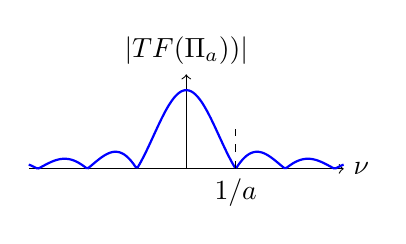
\begin{tikzpicture}
\draw[->] (0,0)--(0,1.2)node[above]{$|TF(\Pi_a ))|$}; 
\draw[->] (-2,0)--(2,0)node[right]{$\nu$};  

\draw[thick,domain=-2:2,color=blue,samples=160] plot (\x,{abs(sin(5*\x r)/(5*\x))});

\draw[dashed] (0.2*3.14,0) node[below]{$1/a$}--(0.2*3.14,0.5);  

\end{tikzpicture}\\
\end{center}
\end{columns} 
\vspace{1 cm}
On va calculer la TFD du signal discret correspondant...
\end{frame}

\begin{frame}
\frametitle{Signal porte} 
On échantillonne le signal porte sur 9 valeurs dont 5 non-nulles
\begin{columns}
\column{60mm}
\begin{center}
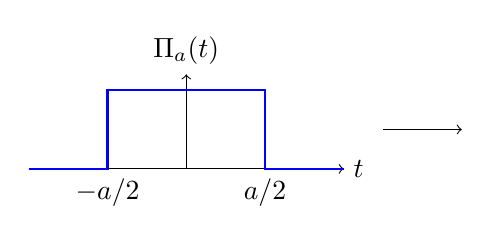
\begin{tikzpicture}
\draw[->] (0,0)--(0,1.2)node[above]{$\Pi_a (t)$}; 
\draw[->] (-2,0)--(2,0)node[right]{$t$};  

\draw[blue,thick] (-2,0)--(-1,0)node[black,below] {$-a/2$}--(-1,1)--(1,1)--(1,0)node[black,below] {$a/2$}--(2,0); 
\draw[->] (2.5,0.5)--(3.5,0.5);
\end{tikzpicture}
\end{center}
\column{60mm}
\begin{center}
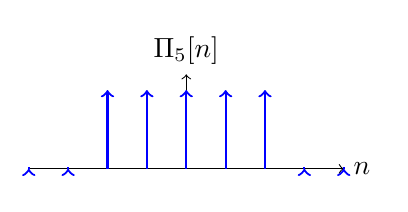
\begin{tikzpicture}
\draw[->] (0,0)--(0,1.2)node[above]{$\Pi_5 [n]$}; 
\draw[->] (-2,0)--(2,0)node[right]{$n$};  

%\draw[blue,thick] (-2,0)--(-1,0)node[black,below] {$-a/2$}--(-1,1)--(1,1)--(1,0)node[black,below] {$a/2$}--(2,0); 
\draw[->,blue,thick] (0,0)--(0,1);
\draw[->,blue,thick] (0.5,0)--(0.5,1);
\draw[->,blue,thick] (-0.5,0)--(-0.5,1);
\draw[->,blue,thick] (1,0)--(1,1);
\draw[->,blue,thick] (-1,0)--(-1,1);
\draw[->,blue,thick] (1.5,0)--(1.5,0);
\draw[->,blue,thick] (-1.5,0)--(-1.5,0);
\draw[->,blue,thick] (2,0)--(2,0);
\draw[->,blue,thick] (-2,0)--(-2,0);
\end{tikzpicture}
\end{center}
\end{columns} 
\only<2->{
\vspace{0.3cm}
On va appliquer la formule de la TFD à ces neufs valeurs.
}
\end{frame}

\begin{frame}
\frametitle{Signal porte} 
\[ \Pi_5[n] = [\; 0 \; 0 \; 1 \; 1 \; 1 \; 1 \; 1 \; 0 \; 0 \;] \] \\
\only<2->{
\vspace{0.5cm}
\[ TFD\{ x \}[m] =  \frac{1}{N} \sum_{k = 0}^{N-1} x[n] \; e^{-j 2 \pi n \frac{m}{N}}  \]\\
\vspace{0.5cm}
}
\only<3->{
\[ TFD\{ \Pi_5 \}[m] = \tilde{\Pi_5}[m]  = \sum_{k = 0}^{8} \Pi_5[k] \; e^{-j 2 \pi k \frac{m}{9}}  \]\\
\vspace{0.5cm}
}
\only<4->{
$m$ indexe les échantillons du spectre résultant du calcul.
}
\end{frame}


\begin{frame}
\frametitle{Signal porte} 
\[ TFD\{ \Pi_5 \}[m] = \tilde{\Pi_5}[m]  = \frac{1}{N} \sum_{k = 0}^{8} \Pi[k] \; e^{-j 2 \pi k \frac{m}{9}}  \]\\
\only<2->{
\vspace{0.5cm}
On somme sur $k$
\[  \tilde{\Pi}[m]  = \frac{1}{9}(  \Pi_5[0] \; e^{-j 2 \pi m \frac{0}{9}}  \; \; + \; \;  \Pi_5[1] \; e^{-j 2 \pi  m \frac{1}{9}} \; \; \; \; + \cdots \; \; \; \; \; +  \Pi_5[8] \; e^{-j 2 \pi m \frac{8}{9}} ) \]\\
}
\only<3->{
\begin{center}
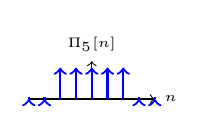
\begin{tikzpicture}
\begin{scope}[scale=0.4]
\draw[->] (0,0)--(0,1.2)node[above]{\tiny{$\Pi_5 [n]$}}; 
\draw[->] (-2,0)--(2,0)node[right]{\tiny{$n$}};  

%\draw[blue,thick] (-2,0)--(-1,0)node[black,below] {$-a/2$}--(-1,1)--(1,1)--(1,0)node[black,below] {$a/2$}--(2,0); 
\draw[->,blue,thick] (0,0)--(0,1);
\draw[->,blue,thick] (0.5,0)--(0.5,1);
\draw[->,blue,thick] (-0.5,0)--(-0.5,1);
\draw[->,blue,thick] (1,0)--(1,1);
\draw[->,blue,thick] (-1,0)--(-1,1);
\draw[->,blue,thick] (1.5,0)--(1.5,0);
\draw[->,blue,thick] (-1.5,0)--(-1.5,0);
\draw[->,blue,thick] (2,0)--(2,0);
\draw[->,blue,thick] (-2,0)--(-2,0);
\end{scope}
\end{tikzpicture}
\end{center}
}
\only<4->{
\[  \tilde{\Pi_5}[m]  =  \frac{1}{9} (  e^{-j 2 \pi  m \frac{2}{9}} +  e^{-j 2 \pi  m \frac{3}{9}} +  e^{-j 2 \pi  m \frac{4}{9}} +  e^{-j 2 \pi  m \frac{5}{9}} + e^{-j 2 \pi  m \frac{6}{9}}) \]
}
\only<5->{
\vspace{0.3cm}
Seuls les échantillons dans la partie non nulle impactent le résultat...
}
\end{frame}
 
\begin{frame}
\frametitle{Signal porte} 
\[  \tilde{\Pi}[m]  =    \frac{1}{9} ( e^{-j 2 \pi  m \frac{2}{9}} +  e^{-j 2 \pi  m \frac{3}{9}} +  e^{-j 2 \pi  m \frac{4}{9}} +  e^{-j 2 \pi  m \frac{5}{9}} + e^{-j 2 \pi  m \frac{6}{9}} ) \]\\
\vspace{0.3cm}

\[  \tilde{\Pi}[0]  =   \frac{1}{9} (  e^{-j 2 \pi  0 \frac{2}{9}} +  e^{-j 2 \pi  0 \frac{3}{9}} +  e^{-j 2 \pi  0 \frac{4}{9}} +  e^{-j 2 \pi  0 \frac{5}{9}} + e^{-j 2 \pi  0 \frac{6}{9}} ) \]\\
\vspace{0.3cm}

\[ \boxed{ \tilde{\Pi}[0]  =   \frac{5}{9} }\]\\
\vspace{0.3cm}

\end{frame}

\begin{frame}
\frametitle{Signal porte} 
\[  \tilde{\Pi}[m]  =    \frac{1}{9} ( e^{-j 2 \pi  m \frac{2}{9}} +  e^{-j 2 \pi  m \frac{3}{9}} +  e^{-j 2 \pi  m \frac{4}{9}} +  e^{-j 2 \pi  m \frac{5}{9}} + e^{-j 2 \pi  m \frac{6}{9}} ) \]\\
\vspace{0.3cm}

\[  \tilde{\Pi}[1]  =   \frac{1}{9} (  e^{-j 2 \pi   \frac{2}{9}} +  e^{-j 2 \pi   \frac{3}{9}} +  e^{-j 2 \pi   \frac{4}{9}} +  e^{-j 2 \pi   \frac{5}{9}} + e^{-j 2 \pi   \frac{6}{9}} ) \]\\
\vspace{0.3cm}
\only<2->{
\[  \tilde{\Pi}[1]  =  \frac{1}{9} ( \scriptsize (0.17-0.98j)  +  (-0.5 -0.87j) +  (-0.94-0.34j)\]
\[ + (-0.94+0.34j) + (-0.5 +0.87j) ) \]
\vspace{0.3cm}
}

\only<3->{
\[ \boxed{ \tilde{\Pi}[1]  =   -0.30 - 0.11j }\]
}
%\vspace{0.3cm}

\end{frame}

\begin{frame}
\frametitle{Signal porte: Amplitude}
On obtient donc les valeurs complexes suivantes pour le spectre 
\begin{columns}
\column{60mm}
\[  \tilde{\Pi_5}[0]  =  0.56 \]
\[  \tilde{\Pi_5}[1]  =   -0.30 - 0.11j \]
\[  \tilde{\Pi_5}[2]  =   -0.04 - 0.04j \]
\[ \tilde{\Pi_5}[3]  =   0.06 + 0.09j \]
\[ \tilde{\Pi_5}[4]  =   0.01 + 0.07j \]
\[ \tilde{\Pi_5}[5]  =   0.01 - 0.07j \]
\[ \tilde{\Pi_5}[6]  =   0.06 - 0.09j \]
\[  \tilde{\Pi_5}[7]  =   -0.04 + 0.04j \]
\[ \tilde{\Pi_5}[8]  =   -0.30 + 0.11j \]
\column{60mm}
\only<2>{
\[  |\tilde{\Pi_5}[0]|  =  0.56 \]
\[  |\tilde{\Pi_5}[1]|  =   0.3195 \]
\[  |\tilde{\Pi_5}[2]|  =   0.05657 \]
\[ |\tilde{\Pi_5}[3]|  =   0.1082 \]
\[ |\tilde{\Pi_5}[4]|  =   0.07071 \]
\[ |\tilde{\Pi_5}[5]|  =   0.07071 \]
\[ |\tilde{\Pi_5}[6]|  =   0.1082 \]
\[  |\tilde{\Pi_5}[7]|  =    0.05657 \]
\[ |\tilde{\Pi_5}[8]|  =   0.3195 \]
}

\end{columns}
\vspace{0.5cm}

\end{frame}

\begin{frame}
\frametitle{Signal porte}
\begin{columns}
\column{60mm}
Module du spectre obtenu par TFD
\begin{center}
\begin{tikzpicture}
\draw[->] (0,0)--(0,3)node[above]{$|\tilde{\Pi_5}|$}; 
\draw[->] (0,0)--(4.5,0)node[right]{$m$};  

\draw[blue,thick] (0,0.55*4)node[left] {0.56}--(0.5,0.32*4)--(1,0.06*4)--(1.5,0.11*4)--(2,0.07*4)--(2.5,0.07*4)--(3,0.11*4)--(3.5,0.06*4)--(4,0.32*4);

\only<3->{
\draw[dashed] (2,0)--(2,3);
}
\end{tikzpicture}
\end{center}
C'est ce que trace MATLAB

\column{60mm}
\only<2-> {\textbf{Comment lire ce spectre ?}}\\
\vspace{0.2cm}
\begin{itemize}
\item 9 points signal =  9 points spectre
\item<3-> Symétrie à partir du 5e échantillon
\item<4-> Fréquences "positives" pour $m \in [0,4]$
\item<5-> Fréquences "négatives" pour $m \in [5,8]$
\end{itemize}
\vspace{0.3cm} 
\only<6->{\textbf{Pourquoi ?}}
\end{columns}
\end{frame}

\begin{frame}
\frametitle{Propriétés des spectres}
On repart de la TF
\only<2->{
\[ TF\{ g\}(\nu) = \tilde{G}(\nu) = \int^{\infty}_{-\infty} g(t) e^{-2\pi j \nu t} \; dt\]\\
\vspace{0.1cm}
définie pour $\nu \in [-\infty,\infty]$\\
}
\only<3->{
\vspace{0.1cm}
Prenons deux fréquences opposées $\nu_0$ et $-\nu_0$,
\[  e^{-2\pi j \nu_0 t} = \cos(-2\pi \nu_0 t) + j \sin(-2\pi \nu_0 t) = \cos(2\pi \nu_0 t) - j \sin(2\pi \nu_0 t) \]
\[  e^{-2\pi j (-\nu_0) t} = e^{2\pi j \nu_0 t} =  \cos(2\pi \nu_0 t) + j \sin(2\pi \nu_0 t) \]\\
\vspace{0.3cm}
}
\only<4->{
Les complexes  $e^{-2\pi j \nu_0 t}$ et  $e^{2\pi j \nu_0 t}$ sont dit \textbf{conjugués} (mêmes parties réelles, parties imaginaires opposées)
}
\end{frame}

\begin{frame}
\frametitle{Propriétés des spectres}
Les complexes  $e^{-2\pi j \nu_0 t}$ et  $e^{2\pi j \nu_0 t}$ sont dit \textbf{conjugués} (mêmes parties réelles, parties imaginaires opposées)\\
\vspace{0.3cm}
\only<2->{
Or, 2 complexes conjugués ont le \textbf{même module}\\
\vspace{0.3cm}
}
\only<3->{
Donc si je reprends TF,
\[\tilde{G}(\nu) = \int^{\infty}_{-\infty} g(t) e^{-2\pi j \nu t} \; dt \rightarrow |\tilde{G}(\nu_0)| = |\tilde{G}(-\nu_0)| \]\\
}
\only<4->{
D'où la symétrie observée pour le spectre en amplitude du signal continu:
\begin{center}
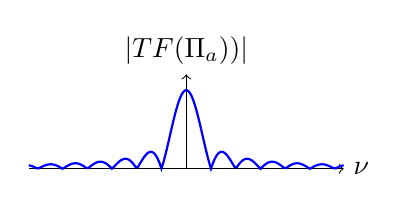
\begin{tikzpicture}
\draw[->] (0,0)--(0,1.2)node[above]{$|TF(\Pi_a ))|$}; 
\draw[->] (-2,0)--(2,0)node[right]{$\nu$};  

\draw[thick,domain=-2:2,color=blue,samples=160] plot (\x,{abs(sin(10*\x r)/(10*\x))});
\end{tikzpicture}\\
\end{center}
}
\end{frame}

\begin{frame}
\frametitle{Propriétés des spectres}
En résumé,
\[\text{Soit } G(\nu) \text{, spectre d'une fonction } g(t). \]
\vspace{0.5cm}
Par définition, $e^{-2\pi j \nu_0 t}$ et  $e^{2\pi j \nu_0 t}$ sont dit \textbf{conjugués} 
\vspace{0.5cm}
\[\tilde{G}(\nu) = \int^{\infty}_{-\infty} g(t) e^{-2\pi j \nu t} \; dt \rightarrow |\tilde{G}(\nu_0)| = |\tilde{G}(-\nu_0)| \]
\vspace{0.5cm}
Donc symétrie de la réponse en amplitude\\
\vspace{0.5cm}
\only<2->{
Et la phase ?
}
\end{frame}

\begin{frame}
\frametitle{Signal porte: Phase}
\begin{columns}
\column{60mm}
\[  \tilde{\Pi_5}[0]  =  0.56 \]
\[  \tilde{\Pi_5}[1]  =   -0.30 - 0.11j \]
\[  \tilde{\Pi_5}[2]  =   -0.04 - 0.04j \]
\[ \tilde{\Pi_5}[3]  =   0.06 + 0.09j \]
\[ \tilde{\Pi_5}[4]  =   0.01 + 0.07j \]
\[ \tilde{\Pi_5}[5]  =   0.01 - 0.07j \]
\[ \tilde{\Pi_5}[6]  =   0.06 - 0.09j \]
\[  \tilde{\Pi_5}[7]  =   -0.04 + 0.04j \]
\[ \tilde{\Pi_5}[8]  =   -0.30 + 0.11j \]
\column{60mm}
\only<2>{
\[  \text{arg}(\tilde{\Pi_5}[0])  =  0 \]
\[ \text{arg}(\tilde{\Pi_5}[1])  =   -2.7901 \]
\[  \text{arg}(\tilde{\Pi_5}[2])  =   -2.3562 \]
\[ \text{arg}(\tilde{\Pi_5}[3])  =   0.9828 \]
\[ \text{arg}(\tilde{\Pi_5}[4])  =   1.4289 \]
\[ \text{arg}(\tilde{\Pi_5}[5])  =   -1.4289 \]
\[ \text{arg}(\tilde{\Pi_5}[6])  =   -0.9828 \]
\[ \text{arg}(\tilde{\Pi_5}[7])  =    2.3562 \]
\[ \text{arg}(\tilde{\Pi_5}[8])  =  2.7901 \]
}
\end{columns}
\end{frame}

\begin{frame}
\frametitle{Signal porte: Phase}
\begin{columns}
\column{60mm}
Module du spectre obtenu par TFD
\begin{center}
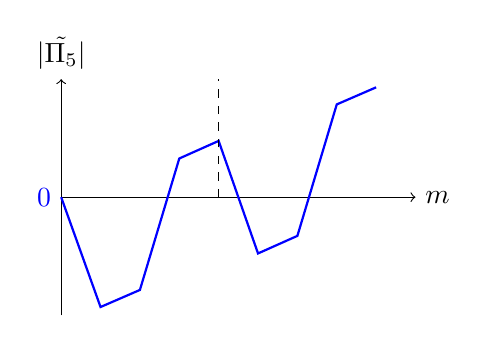
\begin{tikzpicture}
\draw[->] (0,-1.5)--(0,1.5)node[above]{$|\tilde{\Pi_5}|$}; 
\draw[->] (0,0)--(4.5,0)node[right]{$m$};  

\draw[blue,thick] (0,0*4)node[left] {0}--(0.5,-2.79/2)--(1,-2.3562/2)--(1.5,0.9828/2)--(2,1.4289/2)--(2.5,-1.4289/2)--(3,-0.9828/2)--(3.5,2.3562/2)--(4,2.79/2);

\only<3->{
\draw[dashed] (2,0)--(2,1.5);
}
\end{tikzpicture}
\end{center}
C'est ce que trace MATLAB pour $\mathtt{arg(fft(f))}$

\column{60mm}

\begin{itemize}
\item 9 points signal =  9 points spectre
\item<3-> Anti-symétrie des points
\item<4-> Fréquences "positives" pour $m \in [0,4]$
\item<5-> Fréquences "négatives" pour $m \in [5,8]$
\end{itemize}
\end{columns}
\end{frame}

\begin{frame}
\frametitle{Signal Porte : Spectre (TFD)}
En résumé
\begin{center}
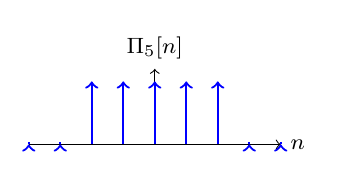
\begin{tikzpicture}
\begin{scope}[scale=0.8]
\draw[->] (0,0)--(0,1.2)node[above]{\footnotesize{$\Pi_5 [n]$}}; 
\draw[->] (-2,0)--(2,0)node[right]{\footnotesize{$n$}};  

%\draw[blue,thick] (-2,0)--(-1,0)node[black,below] {$-a/2$}--(-1,1)--(1,1)--(1,0)node[black,below] {$a/2$}--(2,0); 
\draw[->,blue,thick] (0,0)--(0,1);
\draw[->,blue,thick] (0.5,0)--(0.5,1);
\draw[->,blue,thick] (-0.5,0)--(-0.5,1);
\draw[->,blue,thick] (1,0)--(1,1);
\draw[->,blue,thick] (-1,0)--(-1,1);
\draw[->,blue,thick] (1.5,0)--(1.5,0);
\draw[->,blue,thick] (-1.5,0)--(-1.5,0);
\draw[->,blue,thick] (2,0)--(2,0);
\draw[->,blue,thick] (-2,0)--(-2,0);
\end{scope}
\end{tikzpicture}
\end{center}
\begin{columns}
\column{60mm}
\underline{Amplitude}:
\begin{center}
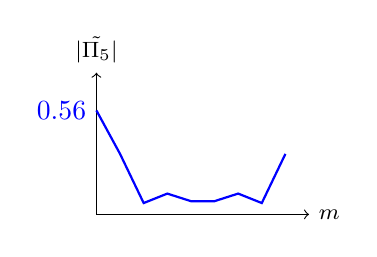
\begin{tikzpicture}
\begin{scope}[scale=0.6]
\draw[->] (0,0)--(0,3)node[above]{\footnotesize{$|\tilde{\Pi_5}|$}}; 
\draw[->] (0,0)--(4.5,0)node[right]{\footnotesize{$m$}};  

\draw[blue,thick] (0,0.55*4)node[left] {0.56}--(0.5,0.32*4)--(1,0.06*4)--(1.5,0.11*4)--(2,0.07*4)--(2.5,0.07*4)--(3,0.11*4)--(3.5,0.06*4)--(4,0.32*4);
\end{scope}

\end{tikzpicture}
\end{center}
\column{60mm}
\underline{Phase}:
\begin{center}
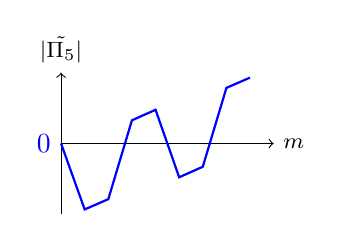
\begin{tikzpicture}
\begin{scope}[scale=0.6]
\draw[->] (0,-1.5)--(0,1.5)node[above]{\footnotesize{$|\tilde{\Pi_5}|$}}; 
\draw[->] (0,0)--(4.5,0)node[right]{\footnotesize{$m$}};  

\draw[blue,thick] (0,0*4)node[left] {0}--(0.5,-2.79/2)--(1,-2.3562/2)--(1.5,0.9828/2)--(2,1.4289/2)--(2.5,-1.4289/2)--(3,-0.9828/2)--(3.5,2.3562/2)--(4,2.79/2);
\end{scope}
\end{tikzpicture}
\end{center}
\end{columns}
\only<2->{
\vspace{0.2cm}
Etudions le lien avec la transformée de Fourier (non-discrète) du signal discret}
\end{frame}


\begin{frame}
\frametitle{Propriétés des spectres}
Pour les signaux discrets, on a :
\[TZ\{ x[n] \} \rightarrow TF\{x[n]\} = \tilde{X}(\nu)  = \sum_{n = -\infty}^{\infty} x[n] e^{-j 2 \pi n \nu T_e}\]\\

On reprend le signal porte précédent,\\

\[TF\{\Pi_5\} = \tilde{\Pi_5}(\nu)  = \sum_{n = -\infty}^{\infty} \Pi_5[n] e^{-j 2 \pi n \nu T_e} = \sum_{n = -2}^{2}  e^{-j 2 \pi n \nu T_e}\]\\

\end{frame}

\begin{frame}
\frametitle{Propriétés des spectres}
\[TF\{\Pi_5\} = \tilde{\Pi_5}(\nu)  = \sum_{n = -\infty}^{\infty} \Pi_5[n] e^{-j 2 \pi n \nu T_e} = \sum_{n = -2}^{2}  e^{-j 2 \pi n \nu T_e}\]\\

\only<2->{
Donc,
\[ TF\{\Pi_5\} = \tilde{\Pi_5}(\nu)= \sum_{n = -2}^{2}  e^{-j 2 \pi n \nu T_e} = 1 + 2 \cos(2\pi \nu T_e) + 2 \cos(4\pi \nu T_e) \]\\
}
\only<3->{
\begin{center}
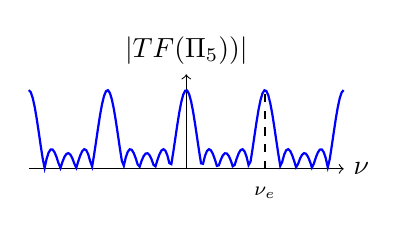
\begin{tikzpicture}
\draw[->] (0,0)--(0,1.2)node[above]{$|TF(\Pi_5 ))|$}; 
\draw[->] (-2,0)--(2,0)node[right]{$\nu$};  

\draw[thick,domain=-2:2,color=blue,samples=160] plot (\x,{0.2*abs(1 + 2*cos(2*3.14*\x r) + 2*cos(4*3.14*\x r)) });

%\draw[dashed,thick,domain=-2:2,color=red,samples=160] plot (\x,{abs(sin(3.14*\x/0.2 r)/(3.14*\x/0.2))});
\only<4->{
\draw[dashed] (1,0)--(1,1);
\draw (1,-0.3) node{\scriptsize{$\nu_e$}};
}

\end{tikzpicture}\\
\end{center}}
\vspace{0.3cm}
\only<4->{
Cette fois-ci le spectre est symétrique ET périodique de période $\nu_e$
}
\end{frame}

\begin{frame}
\frametitle{Propriétés des spectres}
\begin{columns}
\column{60mm}
{\color{blue}\[|TF(\Pi_5 (t))| = \] 
\[ |1 + 2 \cos(2\pi \nu T_e) + 2 \cos(4\pi \nu T_e)|\]}

\column{60mm}
\only<2->{
{\color{red}\[|TF(\Pi_a (t))| =  |\frac{\sin(a \pi\nu)}{\pi\nu}|\]}
}

\end{columns}
\begin{center}
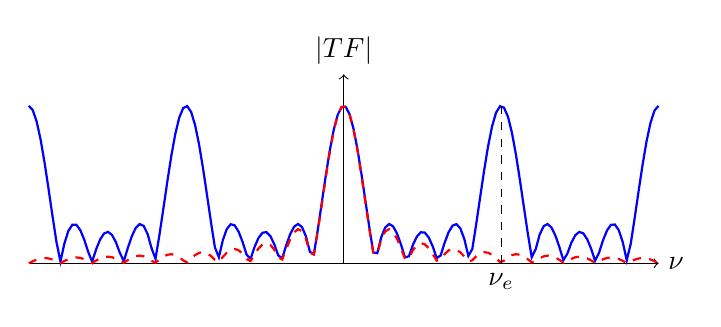
\begin{tikzpicture}
\begin{scope}[scale=2]
\draw[->] (0,0)--(0,1.2)node[above]{$|TF|$}; 
\draw[->] (-2,0)--(2,0)node[right]{$\nu$};  

\draw[thick,domain=-2:2,color=blue,samples=160] plot (\x,{0.2*abs(1 + 2*cos(2*3.14*\x r) + 2*cos(4*3.14*\x r)) });

\only<2->{
\draw[dashed,thick,domain=-2:2,color=red,samples=160] plot (\x,{abs(sin(3.14*\x/0.2 r)/(3.14*\x/0.2))});
}
\draw[dashed] (1,0)node[below]{$\nu_e$}--(1,1);
\end{scope}
\end{tikzpicture}\\
\end{center}
\begin{itemize}
\item<3-> En discrétisant le signal, on a \textbf{périodisé le spectre}
\item<4-> Dans les deux cas, \textbf{symétrie vis-à-vis des fréquences}
\item<5-> Périodicité $\rightarrow$ on ne garde que $[0, \nu_e[$ en discret
\end{itemize}

\end{frame}

\begin{frame}
\frametitle{Propriétés des spectres}
On vient de calculer\\
\[ TF\{\Pi_a\} = \tilde{\Pi_a}(\nu)= \sum_{n = -2}^{2}  e^{-j 2 \pi n \nu T_e} = 1 + 2 \cos(2\pi \nu T_e) + 2 \cos(4\pi \nu T_e) \]\\
\only<2->{
Pour en faire une TFD, il faut échantillonner en fréquence...
} \only<3->{Par \textbf{ convention }
\[ \nu \rightarrow \nu_d = k \Delta f \rightarrow k \frac{1}{N T_e} \;\;\ \text{ avec } k \in [0,N-1] \]\\
}
\only<4->{
Avec cette définition, on a bien :

\[ \nu_d  = k \Delta f \in [0,\frac{(N-1) \nu_e}{N}] \]
}
\end{frame}

%\begin{frame}
%\frametitle{Propriétés des spectres}
%Si on replace les $\nu_d$ dans le graphe précédent\\
%\begin{center}
%\begin{tikzpicture}
%\begin{scope}[scale=2]
%\draw[->] (0,0)--(0,1.2)node[above]{$|TF(\Pi))|$}; 
%\draw[->] (-2,0)--(2,0)node[right]{$\nu$};  
%
%\draw[dashed,thick,domain=-2:2,color=blue,samples=160] plot (\x,{0.2*abs(1 + 2*cos(2*3.14*\x r) + 2*cos(4*3.14*\x r)) });
%
%\draw[dotted,thick,domain=-2:2,color=red,samples=160] plot (\x,{abs(sin(3.14*\x/0.2 r)/(3.14*\x/0.2))});
%
%\only<2>{
%\draw[very thick,domain=0:(6/7),color=blue,samples=7] plot[ycomb] (\x,{0.2*abs(1 + 2*cos(2*3.14*\x r) + 2*cos(4*3.14*\x r)) });
%}
%
%\only<3>{
%\draw[very thick,domain=0:(8/9),color=blue,samples=9] plot[ycomb] (\x,{0.2*abs(1 + 2*cos(2*3.14*\x r) + 2*cos(4*3.14*\x r)) });
%}
%
%
%\draw[dashed] (1,0)node[below]{$\nu_e$}--(1,1);
%\end{scope}
%\end{tikzpicture}\\
%\end{center}
%\begin{itemize}
% \item<2-> On peut placer 7 échantillons en fréquence
% \item<3-> Ou 9...
%\end{itemize}
%\end{frame}


\begin{frame}
\frametitle{Propriétés des spectres}
Si on replace les $\nu_d$ dans le graphe précédent\\
\begin{center}
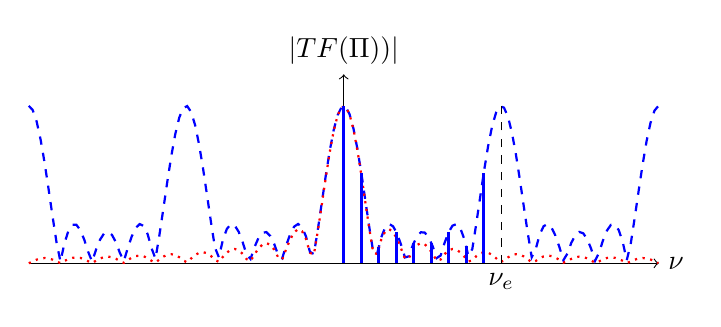
\begin{tikzpicture}
\begin{scope}[scale=2]
\draw[->] (0,0)--(0,1.2)node[above]{$|TF(\Pi))|$}; 
\draw[->] (-2,0)--(2,0)node[right]{$\nu$};  

\draw[dashed,thick,domain=-2:2,color=blue,samples=160] plot (\x,{0.2*abs(1 + 2*cos(2*3.14*\x r) + 2*cos(4*3.14*\x r)) });

\draw[dotted,thick,domain=-2:2,color=red,samples=160] plot (\x,{abs(sin(3.14*\x/0.2 r)/(3.14*\x/0.2))});


\only<2>{
\draw[very thick,domain=0:(8/9),color=blue,samples=9] plot[ycomb] (\x,{0.2*abs(1 + 2*cos(2*3.14*\x r) + 2*cos(4*3.14*\x r)) });
}

\draw[dashed] (1,0)node[below]{$\nu_e$}--(1,1);
\end{scope}
\end{tikzpicture}\\
\end{center}
\begin{itemize}
 \item<2-> On place 9 échantillons en fréquence
\end{itemize}
\end{frame}

\begin{frame}
\frametitle{Propriétés des spectres}
On aurait aussi bien pu décider que\\
\vspace{0.3cm}
 $\nu_d^* = k \Delta f \in [-\nu_e/2, \nu_e/2[$ avec $k \in [-N/2,N/2]$\\
\begin{center}
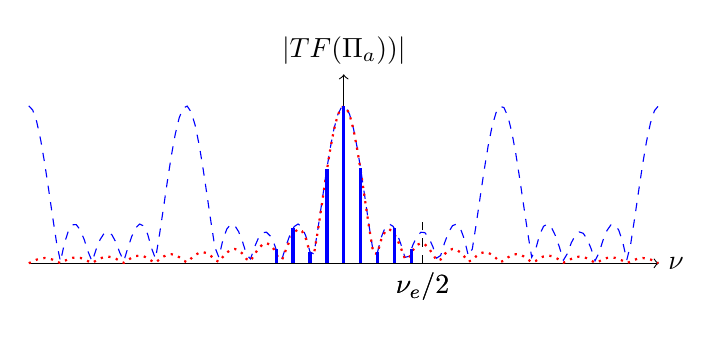
\begin{tikzpicture}
\begin{scope}[scale=2]
\draw[->] (0,0)--(0,1.2)node[above]{$|TF(\Pi_a ))|$}; 
\draw[->] (-2,0)--(2,0)node[right]{$\nu$};  

\draw[dashed,thin,domain=-2:2,color=blue,samples=160] plot (\x,{0.2*abs(1 + 2*cos(2*3.14*\x r) + 2*cos(4*3.14*\x r)) });

\draw[dotted,thick,domain=-2:2,color=red,samples=160] plot (\x,{abs(sin(3.14*\x/0.2 r)/(3.14*\x/0.2))});

\only<2->{
\draw[very thick,domain=-3/7:(3/7),color=blue,samples=9] plot[ycomb] (\x,{0.2*abs(1 + 2*cos(2*3.14*\x r) + 2*cos(4*3.14*\x r)) });
\draw[dashed] (0.5,0)node[below]{$\nu_e/2$}--(0.5,0.3);
\draw[dashed] (0.5,0)node[below]{$\nu_e/2$}--(0.5,0.3);
}



\end{scope}
\end{tikzpicture}\\
\end{center}
\only<3->{
Même information en fréquence au final... \only<4->{Pourquoi avoir choisi l'autre ?}
}
\end{frame}

\begin{frame}
\frametitle{Propriétés des spectres}
Dans le cas $\nu_d  = k \Delta f \in [0,\frac{(N-1) \nu_e}{N}]$, la fréquence nulle est TOUJOURS le premier échantillon du spectre

\begin{center}
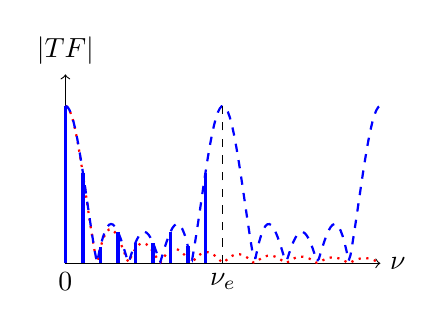
\begin{tikzpicture}
\begin{scope}[scale=2]
\draw[->] (0,0)node[below]{0}--(0,1.2)node[above]{$|TF|$}; 
\draw[->] (0,0)--(2,0)node[right]{$\nu$};  

\draw[dotted,thick,domain=0.001:2,color=red,samples=160] plot (\x,{abs(sin(3.14*\x/0.2 r)/(3.14*\x/0.2))});


\draw[dashed,thick,domain=0:2,color=blue,samples=160] plot (\x,{0.2*abs(1 + 2*cos(2*3.14*\x r) + 2*cos(4*3.14*\x r)) });
\draw[dashed] (1,0)node[below]{$\nu_e$}--(1,1);



\draw[very thick,domain=0:(8/9),color=blue,samples=9] plot[ycomb] (\x,{0.2*abs(1 + 2*cos(2*3.14*\x r) + 2*cos(4*3.14*\x r)) });
\end{scope}
\end{tikzpicture}
\end{center}
\vspace{0.2cm}
\begin{itemize}
\item \'Evite que la position du zéro dépende du nombre d'échantillon
\item Facilite les calculs sur ordi : Indice faible = fréquence faible
\end{itemize}

\end{frame}

\begin{frame}
\frametitle{Propriétés des spectres}
On résume :
\begin{columns}
\column{60mm}
\begin{center}
\begin{tikzpicture}
\begin{scope}[scale=2]
\draw[->] (0,0)--(0,1.2)node[above]{$|TF|$}; 
\draw[->] (0,0)--(2,0)node[right]{$\nu$};  

\draw[dashed,thick,domain=0.001:2,color=red,samples=160] plot (\x,{abs(sin(3.14*\x/0.2 r)/(3.14*\x/0.2))});

\only<2->{
\draw[dotted,thick,domain=0:2,color=blue,samples=160] plot (\x,{0.2*abs(1 + 2*cos(2*3.14*\x r) + 2*cos(4*3.14*\x r)) });
\draw[dashed] (1,0)node[below]{$\nu_e$}--(1,1);
}




\only<3->{
\draw[very thick,domain=0:(8/9),color=blue,samples=9] plot[ycomb] (\x,{0.2*abs(1 + 2*cos(2*3.14*\x r) + 2*cos(4*3.14*\x r)) });
}



\end{scope}
\end{tikzpicture}
\only<3->{
\[ \nu_d \in [0,\frac{(N-1) \nu_e}{N}]\]
}
\end{center}
\column{60mm}
\begin{itemize}
\item Signal continu $\rightarrow$ spectre amplitude \textbf{symétrique}
\vspace{0.3cm}
\item<2-> Signal échantillonné $\rightarrow$ spectre amplitude \textbf{symétrique \& Périodique}
\vspace{0.3cm}
\item<3-> TFD $\rightarrow$ \textbf{échantillonnage arbitraire} du spectre
\vspace{0.3cm}
\item<4-> Echantillonnage "décalé" pour que le premier échantillon du spectre soit la fréquence nulle.
\end{itemize}
\end{columns}
\end{frame}

\subsection{Retour sur le TD MATLAB}
\begin{frame}
\frametitle{Retour sur le TD MATLAB}
\textbf{Résumé }: 
\vspace{0.3cm}
\begin{enumerate}
\item Première prise en main de MATLAB
\vspace{0.3cm}
\item Tracé de la fonction : $g(t) = \cos(2t) + \cos(4t)$
\vspace{0.3cm}
\item Calcul de la transformée de Fourier de $g(t)$
\vspace{0.3cm}
\item Tracé du spectre en amplitude et en phase
\end{enumerate}
\end{frame}


\begin{frame}
\frametitle{Retour sur le TD MATLAB}
\textbf{Tracé de la fonction : $g(t) = \cos(2t) + \cos(4t)$}\\
\vspace{0.3cm}
\begin{columns}
\column{60mm}
\[ g(t) = \cos(2t) + \cos(4t) \]\\
\vspace{0.5cm}
\only<2->{
fonction périodique de période $\pi$\\
}
\vspace{0.5cm}
\only<2->{
On la représente sur $[0, \pi]$
}
\column{60mm}
\only<3->{
\[\mathtt{t = linspace(0,pi,10);}\]
\[\mathtt{>> t = 0, \text{   } 0.3491, \text{   } ... \text{   } 3.1416 }\]
\vspace{0.3cm}
\[\mathtt{g = cos(2*t)+cos(4*t);}\]
\[\mathtt{>> t = 2.0000, \text{   } 0.9397, \text{   } ... \text{   } 2.0000 }\]

\[\mathtt{figure;} \]
\[\mathtt{plot(t,g);}\]

}

\end{columns}
\end{frame}

\begin{frame}
\frametitle{Retour sur le TD MATLAB}
Tracé de la fonction : $g(t) = \cos(2t) + \cos(4t)$\\
\vspace{0.3cm}
\begin{columns}
\column{60mm}

\[\mathtt{t = linspace(0,pi,10);}\]
\[\mathtt{>> t = 0, \text{   } 0.3491, \text{   } ... \text{   } 3.1416 }\]
\vspace{0.3cm}
\[\mathtt{g = cos(2*t)+cos(4*t);}\]
\[\mathtt{>> t = 2.0000, \text{   } 0.9397, \text{   } ... \text{   } 2.0000 }\]

\[\mathtt{figure;} \]
\[\mathtt{plot(t,g);}\]


\column{60mm}
Résultat :

\vspace{0.2cm}

\begin{center}
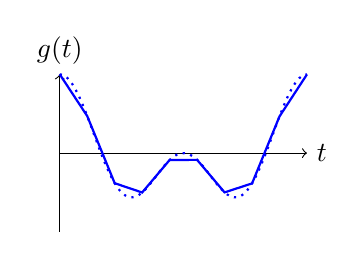
\begin{tikzpicture}

\draw[->] (0,-1)--(0,1)node[above]{$g(t)$}; 
\draw[->] (0,0)--(3.14,0)node[right]{$t$};

\draw[thick,domain=0:3.14,color=blue,samples=10] plot (\x,{0.5*cos(2*\x r) + 0.5*cos(4*\x r)) }) ;
\draw[dotted,thick,domain=0:3.14,color=blue,samples=100] plot (\x,{0.5*cos(2*\x r) + 0.5*cos(4*\x r)) }) ;

\end{tikzpicture}
\end{center} 

\end{columns}
\end{frame}

\begin{frame}
\frametitle{Retour sur le TD MATLAB}
Transformée de Fourier de $g(t) = \cos(2t) + \cos(4t)$\\
\vspace{0.3cm}
\[ G(\nu)\ =  \frac{\delta(\nu+1/\pi) + \delta(\nu-1/\pi)}{2} + \frac{\delta(\nu+2/\pi) + \delta(\nu-2/\pi)}{2}\]
\only<2->{
\begin{columns}
\column{60mm}
\begin{center}
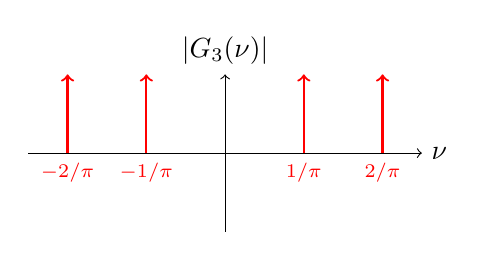
\begin{tikzpicture}
\draw[->] (-2.5,0)--(2.5,0) node[right]{$\nu$};
\draw[->] (0,-1)--(0,1) node[above]{$|G_3(\nu)|$};
\draw[->,red,thick] (-1,0) node[below]{\scriptsize $-1/\pi$}--(-1,1) ;
\draw[->,red,thick] (1,0) node[below]{\scriptsize $1/\pi$}--(1,1) ;
\draw[->,red,thick] (-2,0) node[below]{\scriptsize $-2/\pi$}--(-2,1) ;
\draw[->,red,thick] (2,0) node[below]{\scriptsize $2/\pi$}--(2,1) ;
\end{tikzpicture}
\end{center}
\vspace{0.1cm}
4 diracs
\column{60mm}
\begin{center}
\begin{tikzpicture}
\draw[->] (-2,0)--(2,0) node[right]{$\nu$};
\draw[->] (0,-1)--(0,1) node[above]{$\text{arg}(G_{2,3}(\nu))$};
%\draw[orange,thick] (-1,-1) --(1,1) ;
%\draw[dashed] (-0.65,0)node[above]{\scriptsize -1} --(-0.65,-0.65)--(0,-0.65)node[right]{\scriptsize $-\frac{2\pi^2}{3}$} ;
%\draw[dashed] (0.65,0)node[below]{\scriptsize 1} --(0.65,0.65)--(0,0.65)node[left]{\scriptsize $\frac{2\pi^2}{3}$} ;
\draw[red,thick] (-2,0) --(2,0) ;
\end{tikzpicture}
\end{center}
\vspace{0.1cm}
Phase nulle
\end{columns}
}
\end{frame}

\begin{frame}
\frametitle{Retour sur le TD MATLAB}
TFD
\begin{columns}
\column{60mm}
\begin{itemize}
\item Fréq échantillonnage : $\frac{\displaystyle 9}{\displaystyle \pi}$
\vspace{0.2cm}
\item \'Echantillons fréquence : $k \in [0,9]$\\
\end{itemize}
\vspace{0.2cm}
\textbf{Important:} Enlever le dernier point pour éviter une répétition source de parasites

\column{60mm}
\[\mathtt{tfg = fft(g(1:9));}\]
\[\mathtt{N = 10;}\]
\vspace{0.3cm}
\[\mathtt{fe = 9/pi;}\]
\[\mathtt{f = linspace(0,(N-1)./N*df,10);}\]

\[\mathtt{figure;} \]
\[\mathtt{plot(f,abs(tfg));}\]
\end{columns}
\end{frame}

\begin{frame}
\frametitle{Retour sur le TD MATLAB}
TFD
\begin{columns}

\column{60mm}
\[\mathtt{tfg = fft(g(1:9));}\]
\[\mathtt{N = 10;}\]
\vspace{0.3cm}
\[\mathtt{fe = 9/pi;}\]
\[\mathtt{f = linspace(0,(N-1)./N*fe,N);}\]

\[\mathtt{figure;} \]
\[\mathtt{plot(f,abs(tfg(1:9)));}\]

\column{60mm}
Résultat:\\
\vspace{0.2cm}
\begin{center}
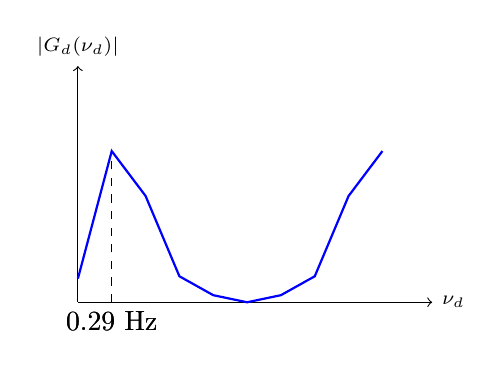
\begin{tikzpicture}
\begin{scope}[scale=1.5]
\draw[->] (0,0)-- (3,0)node[right] {\scriptsize $\nu_d$} ;
\draw[->] (0,0)-- (0,2)node[above] {\scriptsize $|G_d(\nu_d)|$};
\draw[thick,blue] plot coordinates{
(0,0.2)
(0.2865,2*0.64)
(0.5730,2*0.45)
(0.8594,2*0.11)
(1.1459,2*0.03)
(1.4324,0)
(1.7189,2*0.03)
(2.0054,2*0.11)
(2.2918,2*0.45)
(2.5783,2*0.64)
};
\draw[dashed] (0.2865,0)node[below]{0.29 Hz}--(0.2865,2*0.64);
\draw[dashed] (0.2865,0)node[below]{0.29 Hz}--(0.2865,2*0.64);
\end{scope}
\end{tikzpicture}
\end{center}
\only<3->{
On ne dispose que de 10 points de spectre avec ce code...
}
\end{columns}
\end{frame}

\begin{frame}
\frametitle{Retour sur le TD MATLAB}
On change le code pour avoir plus de points :\\
\vspace{0.2cm}
\begin{columns}

\column{60mm}
Rappel : $N_{pts,spectre} = N_{pts,signal}$ est une convention de calcul \\
\vspace{0.3cm}
\begin{itemize}
\item Rajouter des points au spectre ne change pas $f_e$ ni $\Delta_f$
\vspace{0.2cm}
\item On rééchantillonne le spectre sans toucher au signal
\end{itemize}
 

\column{60mm}
\[\mathtt{tfg2 = fft(g(1:9),100);}\]
\[\mathtt{N = 100;}\]
\vspace{0.3cm}
\[\mathtt{fe = 9/pi;}\]
\[\mathtt{f = linspace(0,(N-1)./N*df,N);}\]

\[\mathtt{figure;} \]
\[\mathtt{plot(f,abs(tfg2));}\]

\end{columns}
\end{frame}

\begin{frame}
\frametitle{Retour sur le TD MATLAB}
On change le code pour avoir plus de points :\\
\vspace{0.2cm}
\begin{columns}

\column{60mm}
\[\mathtt{tfg2 = fft(g(1:9),100);}\]
\[\mathtt{N = 100;}\]
\vspace{0.3cm}
\[\mathtt{df = 9/pi;}\]
\[\mathtt{f = linspace(0,(N-1)./N*df,N);}\]

\[\mathtt{figure;} \]
\[\mathtt{plot(f,abs(tfg2));}\]

\column{60mm}
Résultat:\\
\vspace{0.2cm}
\begin{center}
\begin{tikzpicture}
\begin{scope}[scale=1.5]
\draw[->] (0,0)-- (3,0)node[right] {\scriptsize $\nu_d$} ;
\draw[->] (0,0)-- (0,2)node[above] {\scriptsize $|G_d(\nu_d)|$};
\draw[thick,blue] plot file {module_cos2freq_100pts.txt};

\draw[dashed] (0.29,0)node[below]{ \scriptsize 0.29 Hz}--(0.29,2*0.64);
\draw[dashed] (0.72,0)--(0.72,2*0.64) node[above]{\scriptsize 0.72 Hz};
\end{scope}
\end{tikzpicture}
\end{center}
\only<2->{
Les lobes sont toujours décalés en fréquence...
}
\end{columns}
\end{frame}
%Enchaîner sur la périodisation du signal tempo

\begin{frame}
\frametitle{Retour sur le TD MATLAB}
On résume  :\\
\vspace{0.2cm}
\begin{columns}
\column{60mm}
Spectre d'une période de $g(t) = \cos(2t)+\cos(4t)$
\vspace{0.2cm}
\begin{center}
\begin{tikzpicture}
\begin{scope}[scale=1.5]
\draw[->] (0,0)-- (3,0)node[right] {\scriptsize $\nu_d$} ;
\draw[->] (0,0)-- (0,2)node[above] {\scriptsize $|G_d(\nu_d)|$};
\draw[thick,blue] plot file {module_cos2freq_100pts.txt};

\draw[dashed] (0.29,0)node[below]{ \scriptsize 0.29 Hz}--(0.29,2*0.64);
\draw[dashed] (0.72,0)--(0.72,2*0.64) node[above]{\scriptsize 0.72 Hz};
\end{scope}
\end{tikzpicture}
\end{center}
\column{60mm}
Observations: \\
\vspace{0.3cm}
\begin{itemize}
\item<2-> Signal temporel sur 10 pts
\vspace{0.3 cm}
\item<3-> Spectre sur 10 points difficile à lire $\rightarrow$ on passe sur 100 pts
\vspace{0.3 cm}
\item<4-> Lobes décalés en fréq par rapport au spectre "réel"
\end{itemize}
\vspace{0.3 cm}
\only<5->{
\textbf{Pourquoi ?}
}
\end{columns}
\end{frame}

\begin{frame}
\frametitle{Retour sur le TD MATLAB}
\begin{columns}
\column{60mm}
Le signal "complet"
\begin{center}
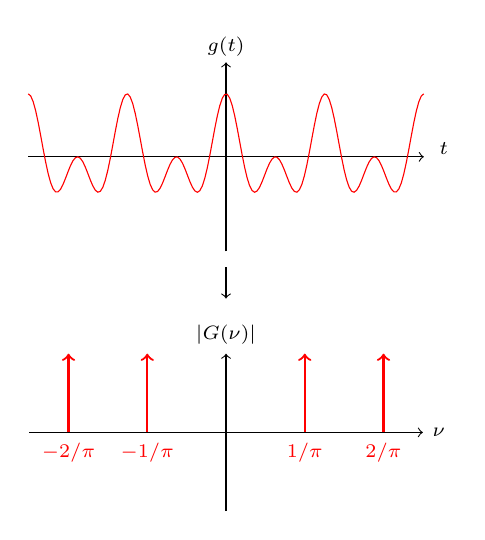
\begin{tikzpicture}
	\begin{scope}[scale=0.4]
	\draw[->] (-6.28,0)-- (6.28,0);
%\draw (-0.3,-0.3) node {0};
\draw[->] (0,-3)-- (0,3);
\draw (2.2*pi,0.25) node {\scriptsize $t$};
\draw (0,3.5) node {\scriptsize $g(t)$};

	\draw[domain=-6.28:6.28,color=red,samples=160] plot (\x,{(cos(2*\x r)+ cos(2*2*\x r))});
	
	%	\draw[domain=-6.28:6.28,color=orange,samples=160] plot (\x,{2*(0.55*cos(2*\x r)+ 0.45*cos(2*2*(\x+3.14/12) r))});
\only<2->{	
	\draw[->] (0,-3.5)--(0,-4.5);
}	
	\end{scope}
\only<2->{		
\begin{scope}[yshift=-3.5cm]
\draw[->] (-2.5,0)--(2.5,0) node[right]{\scriptsize $\nu$};
\draw[->] (0,-1)--(0,1) node[above]{\scriptsize $|G(\nu)|$};
\draw[->,red,thick] (-1,0) node[below]{\scriptsize $-1/\pi$}--(-1,1) ;
\draw[->,red,thick] (1,0) node[below]{\scriptsize $1/\pi$}--(1,1) ;
\draw[->,red,thick] (-2,0) node[below]{\scriptsize $-2/\pi$}--(-2,1) ;
\draw[->,red,thick] (2,0) node[below]{\scriptsize $2/\pi$}--(2,1) ;
\end{scope}
}
	\end{tikzpicture}
\end{center}

\column{60mm}
\only<3->{
 \small dans MATLAB, signal échantillonné \textbf{ET fenêtré}
\begin{center}
\begin{tikzpicture}
	\begin{scope}[scale=0.4,yshift=2cm]
	\draw[->] (-6.28,0)-- (6.28,0);
%\draw (-0.3,-0.3) node {0};
\draw[->] (0,-3)-- (0,3);
\draw (2.2*pi,0.25) node {\scriptsize $t$};
\draw (0,3.5) node {\scriptsize $g(t)$};

	\draw[domain=0:3.14,color=blue,samples=9] plot (\x,{(cos(2*\x r)+ cos(2*2*\x r))});
		\draw[dotted,domain=-6.28:6.28,color=red,samples=160] plot (\x,{(cos(2*\x r)+ cos(2*2*\x r))});
	
	%	\draw[domain=-6.28:6.28,color=orange,samples=160] plot (\x,{2*(0.55*cos(2*\x r)+ 0.45*cos(2*2*(\x+3.14/12) r))});
\only<4->{	
	\draw[->] (0,-3.5)--(0,-4.5);
}	
	\end{scope}
\only<4->{		
\begin{scope}[scale=0.9,yshift=-3.5cm]
\draw[->] (-3,0)-- (3,0)node[right] {\scriptsize $\nu_d$} ;
\draw[->] (0,-1.5)-- (0,1.5)node[above] {\scriptsize $|G_d(\nu_d)|$};
\draw[thick,blue] plot file {module_cos2freq_100pts.txt};

%\draw[dashed] (0.29,0)node[below]{ \scriptsize 0.29 Hz}--(0.29,2*0.64);
%\draw[dashed] (0.72,0)--(0.72,2*0.64) node[above]{\scriptsize 0.72 Hz};
\end{scope}
}
	\end{tikzpicture}
\end{center}
}
\end{columns}
\end{frame}

\begin{frame}
\frametitle{Retour sur le TD MATLAB}
\begin{columns}

\column{60mm}
 \small On résume
\begin{center}
\begin{tikzpicture}
	\begin{scope}[scale=0.4,yshift=2cm]
	\draw[->] (-6.28,0)-- (6.28,0);
%\draw (-0.3,-0.3) node {0};
\draw[->] (0,-3)-- (0,3);
\draw (2.2*pi,0.25) node {\scriptsize $t$};
\draw (0,3.5) node {\scriptsize $g(t)$};

	\draw[domain=0:3.14,color=blue,samples=9] plot (\x,{(cos(2*\x r)+ cos(2*2*\x r))});
		\draw[dotted,domain=-6.28:6.28,color=red,samples=160] plot (\x,{(cos(2*\x r)+ cos(2*2*\x r))});
	
	%	\draw[domain=-6.28:6.28,color=orange,samples=160] plot (\x,{2*(0.55*cos(2*\x r)+ 0.45*cos(2*2*(\x+3.14/12) r))});
	
	\draw[->] (0,-3.5)--(0,-4.5);
	
	\end{scope}
	
\begin{scope}[scale=0.9,yshift=-3.5cm]
\draw[->] (-3,0)-- (3,0)node[right] {\scriptsize $\nu_d$} ;
\draw[->] (0,-1.5)-- (0,1.5)node[above] {\scriptsize $|G_d(\nu_d)|$};
\draw[thick,blue] plot file {module_cos2freq_100pts.txt};

%\draw[dashed] (0.29,0)node[below]{ \scriptsize 0.29 Hz}--(0.29,2*0.64);
%\draw[dashed] (0.72,0)--(0.72,2*0.64) node[above]{\scriptsize 0.72 Hz};
\end{scope}

	\end{tikzpicture}
\end{center}

\column{60mm}
\begin{itemize}
\item Signal MATLAB =  signal réel échantillonné et fenêtré 
\vspace{0.2cm}
\item<2-> Echantillonnage =  Périodisation du spectre 
\vspace{0.2cm}
\item<3-> Fenêtrage = Apparition de lobes 
\end{itemize}
\vspace{0.2cm}
\only<4->{
Spectre initial "déformé" par le passage en MATLAB\\
\vspace{0.3cm}
}
\only<5->{
\textbf{Solution ?}
}
\end{columns}

\end{frame}

\begin{frame}
\frametitle{Retour sur le TD MATLAB}
\small On change le code pour avoir une fenêtre plus large :\\
\vspace{0.1cm}
\begin{columns}

\column{60mm}
\[\mathtt{t = linspace(0,8*pi,80);}\]
\[\mathtt{g2 = cos(2*t)+cos(4*t);}\]
\[\mathtt{tfg2 = fft(g2(1:79),100);}\]
\[\mathtt{N = 100;}\]

\[\mathtt{fe = 79/8*pi;}\]
\[\mathtt{f = linspace(0,(N-1)./N*fe,N);}\]

\[\mathtt{figure;} \]
\[\mathtt{plot(f,abs(tfg2));}\]

\column{60mm}
Résultat:\\
\vspace{0.2cm}
\begin{center}
\begin{tikzpicture}

\begin{scope}[scale=1.5]
\draw[->] (0,0)-- (3,0)node[right] {\scriptsize $\nu_d$} ;
\draw[->] (0,0)-- (0,2)node[above] {\scriptsize $|G_d(\nu_d)|$};
\draw[thick,blue] plot file {mod_cos2freq_100pts.txt};

\draw[dashed] (1/3.14,0)node[below]{ \scriptsize 0.32 Hz}--(1/3.14,2*0.8);
\draw[dashed] (2/3.14,0)--(2/3.14,2*0.8) node[above]{\scriptsize 0.64 Hz};
\end{scope}
\end{tikzpicture}
\end{center}

\end{columns}
\end{frame}

\begin{frame}
\frametitle{Retour sur le TD MATLAB}

\begin{columns}

\column{60mm}

\vspace{0.2cm}
\begin{center}
\begin{tikzpicture}

\begin{scope}[scale=1.5]
\draw[->] (0,0)-- (3,0)node[right] {\scriptsize $\nu_d$} ;
\draw[->] (0,0)-- (0,2)node[above] {\scriptsize $|G_d(\nu_d)|$};
\draw[thick,blue] plot file {mod_cos2freq_100pts.txt};

\draw[dashed] (1/3.14,0)node[below]{ \scriptsize 0.32 Hz}--(1/3.14,2*0.8);
\draw[dashed] (2/3.14,0)--(2/3.14,2*0.8) node[above]{\scriptsize 0.64 Hz};
\end{scope}
\end{tikzpicture}
\end{center}

\column{60mm}
On résume :\\
\vspace{0.2cm}
\begin{itemize}
\item On passe d'une fenêtre temporelle de  1 à 8 périodes
\vspace{0.2cm}
\item La fenêtre temporelle plus large "réduit" les lobes
\vspace{0.2cm}
\item Les pics sont mieux définis $\rightarrow$ plus proche du signal réel périodique
 
\end{itemize}
\end{columns}
\end{frame}

\begin{frame}
\frametitle{Retour sur le TD MATLAB}
\textbf{\underline{Résumé global}}:
\vspace{0.2cm}
\begin{enumerate}
\item \textbf{Convention de représentation des spectres dans MATLAB} 
\begin{itemize}
\item $\nu_d \in [0, \nu_e]$
\vspace{0.15cm}
\item fréquence nulle = 1er échantillon
\end{itemize}
\vspace{0.2cm}
\item \textbf{Tracé du spectre de $g(t) = \cos(2t)+\cos(4t)$}
\begin{itemize}
\item tracé spectre 1 période = lobes importants et décalés
\vspace{0.15cm}
\item tracé spectre 8 périodes = pics mieux définis et mieux placés 
\end{itemize}
\vspace{0.2cm}
\item \textbf{Spectre dans MATLAB = spectre signal échantillonné ET fenêtré}
\begin{itemize}
\item échantillonnage signal = périodisation spectre
\vspace{0.15cm}
\item fenêtrage signal = apparition de lobes 
\begin{itemize}
\vspace{0.15cm}
\item fenêtre courte = lobes importantes
\vspace{0.15cm}
\item fenêtre large = lobes moins prononcés
\end{itemize}
\end{itemize}
\end{enumerate}
\end{frame}
\end{document}